% Created 2022-07-30 Sat 15:50
% Intended LaTeX compiler: pdflatex
\documentclass[smaller, aspectratio=1610]{beamer}
\usepackage[utf8]{inputenc}
\usepackage[T1]{fontenc}
\usepackage{graphicx}
\usepackage{longtable}
\usepackage{wrapfig}
\usepackage{rotating}
\usepackage[normalem]{ulem}
\usepackage{amsmath}
\usepackage{amssymb}
\usepackage{capt-of}
\usepackage{hyperref}
\setbeamertemplate{navigation symbols}{}
\usepackage{verbatim, multicol, tabularx}
\usepackage{sourcecodepro}
\usepackage[T1]{fontenc}
\usepackage{amsmath,amsthm, amssymb, latexsym, listings, qtree}
\lstset{extendedchars=\true, inputencoding=utf8, frame=tb, aboveskip=1mm, belowskip=0mm, showstringspaces=false, columns=fixed, basicstyle={\footnotesize\ttfamily}, numbers=left, frame=single, breaklines=true, breakatwhitespace=true, tabsize=4,  keywordstyle=\color{blue}, identifierstyle=\color{violet}, stringstyle=\color{teal}, commentstyle=\color{darkgray}}
\setbeamertemplate{footline}[frame number]
\hypersetup{colorlinks=true,urlcolor=blue,bookmarks=true}
\setlength{\parskip}{.25\baselineskip}
\usetheme{default}
\date{}
\title{Functions}
\hypersetup{
 pdfauthor={},
 pdftitle={Functions},
 pdfkeywords={},
 pdfsubject={},
 pdfcreator={Emacs 28.1 (Org mode 9.5.2)},
 pdflang={English}}
\begin{document}

\maketitle

\section{Functions}
\label{sec:org2bbeba0}

\begin{frame}[label={sec:org237e2a8}]{Functions}
A function is a reusable block of code. Functions

\begin{itemize}
\item have names (usually),
\item contain a sequence of statements, and
\item return values, either explicitly or implicitly.
\end{itemize}

We've already used several built-in functions. Today we will learn how to define our own.
\end{frame}

\begin{frame}[label={sec:org5ce04a4},fragile]{Hello, Functions!}
 We define a function using the def keyword:

\lstset{language=Python,label= ,caption= ,captionpos=b,numbers=none}
\begin{lstlisting}
>>> def greet():
...     print('Hello')
...
\end{lstlisting}

(blank line tells Python shell you're finished defining the function)

Once the function is defined, you can call it:

\lstset{language=Python,label= ,caption= ,captionpos=b,numbers=none}
\begin{lstlisting}
>>> greet()
Hello
\end{lstlisting}

> What happens if you evaluate \texttt{greet} (without the \texttt{()}) in the Python REPL?
\end{frame}

\begin{frame}[label={sec:org2ac6e11},fragile]{Defining Functions}
 The general form of a function definition is

\lstset{language=Python,label= ,caption= ,captionpos=b,numbers=none}
\begin{lstlisting}
def <function_name>(<parameter_list>):
    <function_body>
\end{lstlisting}

\begin{itemize}
\item The first line is called the header.
\item \texttt{function\_name} is the name you use to call the function.
\item \texttt{parameter\_list} is a list of parameters to the function, which may be empty.
\item \texttt{function\_body} is a sequence of expressions and statements.
\end{itemize}
\end{frame}

\begin{frame}[label={sec:org4b2652d},fragile]{Function Parameters}
 Provide a list of parameter names inside the parentheses of the function header, which creates local variables in the function.

\lstset{language=Python,label= ,caption= ,captionpos=b,numbers=none}
\begin{lstlisting}
>>> def greet(name):
        g = "Hello, " + name + "!"
...     print(g)
...
\end{lstlisting}

Then call the function by passing \alert{arguments} to the function: values that are bound to parameter names.

Here we pass the value 'Hello', which is bound to \texttt{greet}'s parameter \texttt{name} and printed to the console by the code inside \texttt{greet}.

\lstset{language=Python,label= ,caption= ,captionpos=b,numbers=none}
\begin{lstlisting}
>>> greet('Dolly')
Hello, Dolly!
\end{lstlisting}
\end{frame}

\begin{frame}[label={sec:org49537f8},fragile]{Function Call Semantics}
 \begin{columns}
\begin{column}{0.3\columnwidth}
\begin{block}{}
\lstset{language=Python,label= ,caption= ,captionpos=b,numbers=none}
\begin{lstlisting}
>>> g = "Dolly"
\end{lstlisting}

Creates a global value\footnote{Since \texttt{str} is a sequence data structure, this memory image is a slight simplification.}.

\begin{center}
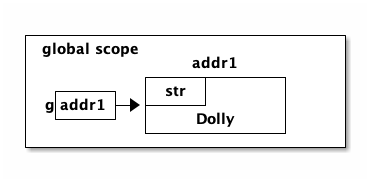
\includegraphics[width=1.75in]{diagrams/dolly.png}
\end{center}
\end{block}
\end{column}

\begin{column}{0.3\columnwidth}
\begin{block}{}
\lstset{language=Python,label= ,caption= ,captionpos=b,numbers=none}
\begin{lstlisting}
>>> greet(g)
\end{lstlisting}

Passes argument \texttt{g} \emph{by value}, that is, the object pointer in \texttt{g} is copied to \texttt{greet}'s \texttt{name} parameter.

\begin{center}
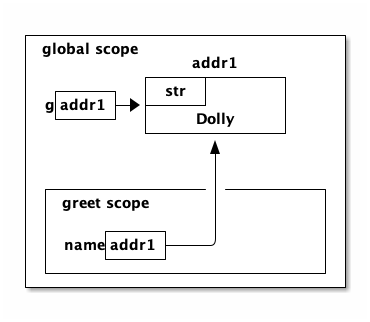
\includegraphics[width=1.75in]{diagrams/greet-dolly.png}
\end{center}
\end{block}
\end{column}


\begin{column}{0.3\columnwidth}
\begin{block}{}
\lstset{language=Python,label= ,caption= ,captionpos=b,numbers=none,basicstyle=\ttfamily\scriptsize, numbers=left}
\begin{lstlisting}
def greet(name):
    g = "Hello, "+name+"!"
    print(g)
\end{lstlisting}

Notice that \texttt{greet}'s \texttt{g} shadows the global \texttt{g}.
\begin{center}
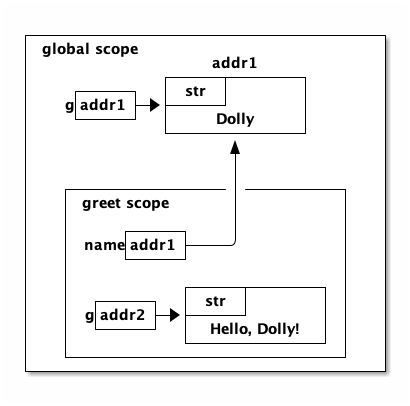
\includegraphics[width=1.75in]{diagrams/greet-scoppe.png}
\end{center}
\end{block}
\end{column}
\end{columns}
\end{frame}


\begin{frame}[label={sec:orgab0c48c},fragile]{Strict Argument Evaluation}
 Arguments to functions are evaluated strictly, meaning that they are evaluated before control is transferred to the function body.

Here we pass the value 'Guten Tag!':

\lstset{language=Python,label= ,caption= ,captionpos=b,numbers=none}
\begin{lstlisting}
>>> greet('Guten Tag!')
Guten Tag!
\end{lstlisting}
\end{frame}

\begin{frame}[label={sec:org57f5c3e},fragile]{Variable Scope}
 Parameters are local variables. They are not visible outside the function:

\lstset{language=Python,label= ,caption= ,captionpos=b,numbers=none}
\begin{lstlisting}
>>> name
Traceback (most recent call last):
  File "<stdin>", line 1, in <module>
NameError: name 'name' is not defined
\end{lstlisting}

Global variables are visible outside the function and inside the function.

\lstset{language=Python,label= ,caption= ,captionpos=b,numbers=none}
\begin{lstlisting}
>>> global_hello = 'Bonjour'
>>> global_hello
'Bonjour'
>>> def say_global_hello():
...     print(global_hello)
...
>>> say_global_hello()
Bonjour
\end{lstlisting}
\end{frame}

\begin{frame}[label={sec:org163e2ff},fragile]{Shadowing Global Variables}
 Local variables shadow global variables.

\lstset{language=Python,label= ,caption= ,captionpos=b,numbers=none}
\begin{lstlisting}
>>> x = 1
>>> def f():
...     x = 2
...     print("local x:", x)
...     print("global x:", globals()["x"])
...
>>> f()
local x: 2
global x: 1
\end{lstlisting}

\begin{itemize}
\item Tip: evaluate \texttt{globals()["\_\_name\_\_"]} in the Python REPL.
\end{itemize}

A function parameter is a local variable.

\lstset{language=Python,label= ,caption= ,captionpos=b,numbers=none}
\begin{lstlisting}
>>> name = 'Hi ya!'
>>> def greet(name):
...     print(name)
...
>>> name
'Hi ya!'
>>> greet('Hello')
Hello
\end{lstlisting}
\end{frame}

\begin{frame}[label={sec:org43668d5},fragile]{Namespaces}
 Every place where a variable can be defined is called a \alert{namespace} or a \alert{frame} (sometimes also called a \alert{symbol table}, which is how namespaces are implemented by compilers and interpreters).

\begin{itemize}
\item Top level, or \alert{global} names (either the Python REPL or a script) are in a namespace called \texttt{\_\_main\_\_}.
\item Each function \alert{call} also gets a namespace for the local variables in the function.
\item These namespaces are hierarchical -- name resolution starts with the innermost namespace, which is why local variables "hide" or "shadow" global variables.
\end{itemize}
\end{frame}

\begin{frame}[label={sec:org6bfde85}]{Memory Model With Function Calls}
\end{frame}

\begin{frame}[label={sec:orgca768ed},fragile]{Redefining Names}
 A function a kind of variable. If you define a function with the same name as a variable, it re-binds the name, and vice-versa.

\lstset{language=Python,label= ,caption= ,captionpos=b,numbers=none}
\begin{lstlisting}
>>> global_hello = 'Bonjour'
>>> def global_hello():
...     print('This is the global_hello() function.')
...
>>> global_hello
<function global_hello at 0x10063b620>
\end{lstlisting}
\end{frame}

\begin{frame}[label={sec:org2738701}]{Python Scope Gotchas}
Python has notoriously weird scoping rules.
\end{frame}

\begin{frame}[label={sec:org3105715},fragile]{Muliple Parameters}
 A function can take any number of parameters.

\lstset{language=Python,label= ,caption= ,captionpos=b,numbers=none}
\begin{lstlisting}
>>> def greet(name, name):
...     print(name + ', ' + name)
...
>>> greet('Professor Falken', 'Greetings')
Greetings, Professor Falken
\end{lstlisting}

Parameters can be of multiple types.

\lstset{language=Python,label= ,caption= ,captionpos=b,numbers=none}
\begin{lstlisting}
>>> def greet(name, name, number):
...     print(name * number + ', ' + name)
...
>>> greet('Professor Falken', 'Greetings', 2)
GreetingsGreetings, Professor Falken
\end{lstlisting}
\end{frame}

\begin{frame}[label={sec:org0f4b20f},fragile]{Positional and Keyword Arguments}
 Thus far we've called functions using positional arguments, meaning that argument values are bound to parameters in the order in which they appear in the call.

\lstset{language=Python,label= ,caption= ,captionpos=b,numbers=none}
\begin{lstlisting}
>>> def greet(name, name, number):
...     print(name * number + ', ' + name)
...
>>> greet('Professor Falken', 'Greetings', 2)
\end{lstlisting}

We can also call functions with keyword arguments in any order.

\lstset{language=Python,label= ,caption= ,captionpos=b,numbers=none}
\begin{lstlisting}
>>> greet(name='Hello', number=2, name='Dolly')
HelloHello, Dolly
\end{lstlisting}

If you call a function with both positional and keyword arguments, the positional ones must come first.
\end{frame}

\begin{frame}[label={sec:org9bf082c},fragile]{Default Parameter Values}
 You can specify default parameter values so that you don't have to provide an argument.

\lstset{language=Python,label= ,caption= ,captionpos=b,numbers=none}
\begin{lstlisting}
>>> def greet(name, name='Hello'):
...     print(name + ', ' + name)
...
>>> greet('Elmo')
Hello, Elmo
\end{lstlisting}

If you provide an argument for a parameter with a default value, the parameter takes the argument value passed in the call instead of the default value.

\lstset{language=Python,label= ,caption= ,captionpos=b,numbers=none}
\begin{lstlisting}
>>> greet('Elmo', 'Hi')
Hi, Elmo
\end{lstlisting}
\end{frame}

\begin{frame}[label={sec:org3be8e48},fragile]{Return Values}
 Functions return values.

\lstset{language=Python,label= ,caption= ,captionpos=b,numbers=none}
\begin{lstlisting}
>>> def double(num):
...     return num * 2
...
>>> double(2)
4
\end{lstlisting}

If you don't explicitly return a value, \texttt{None} is returned implicitly.

\lstset{language=Python,label= ,caption= ,captionpos=b,numbers=none}
\begin{lstlisting}
>>> def g():
...     print("man") # This is not a return!
...
>>> fbi = g()
man # This is a side-effect of calling g(), not a return value
>>> type(fbi)
<class 'NoneType'>
\end{lstlisting}

Function calls are expressions like any other, that is, a function call has a value, so a function call can appear anywhere a value can appear.

\lstset{language=Python,label= ,caption= ,captionpos=b,numbers=none}
\begin{lstlisting}
>>> double(2) + double(3)
10
\end{lstlisting}
\end{frame}

\begin{frame}[label={sec:org7050158}]{Function Design Recipe}
\begin{enumerate}
\item Examples
\begin{itemize}
\item What a few representative calls to the function look like in the Python REPL.
\begin{itemize}
\item Think from the function \alert{user's} perspective.
\item Examples become doctests in the function's docstring.
\end{itemize}
\end{itemize}

\item Header
\begin{itemize}
\item Parameter names and types
\item Return type
\end{itemize}

\item Description
\begin{itemize}
\item Short paragraph (1 or 2 sentences) describing the function's behavior.
\end{itemize}

\item Body
\begin{itemize}
\item Implement the algorithm (sequence of statements) that accomplishes the function's task, deriving the function's output (return value) and/or effect from the the function's inputs (arguments).
\end{itemize}

\item Test
\begin{itemize}
\item Test your function on some representative inputs (try to include edge cases).
\end{itemize}
\end{enumerate}
\end{frame}


\begin{frame}[label={sec:org922e455},fragile]{Writing Function Examples}
 Let's apply this design recipe in the creation of a simple function to calculate the length of the hypotenuse from the lengths of the two legs (the sides that join in a right angle).

First, decide the name of the function.

\begin{itemize}
\item Descriptive word(s)
\begin{itemize}
\item Verbs may imply an imperative function called for its effect, not a return value
\begin{itemize}
\item \texttt{print("hello")}, \texttt{exit()}
\end{itemize}
\item Nouns may imply a pure function, a return value derived only from the function's arguments with no side effects
\begin{itemize}
\item \texttt{type(1)}, \texttt{double(2)}
\end{itemize}
\end{itemize}

\item Avoid Python keywords or names of library functions.
\begin{itemize}
\item Tip:

\lstset{language=Python,label= ,caption= ,captionpos=b,numbers=none}
\begin{lstlisting}
        >>> import keyword
        >>> keyword.kwlist # lists all the Python keywords
        >>> keyword.iskeyword("foo") # True if "foo" is a keyword
\end{lstlisting}
\end{itemize}

\item Follow Python's \href{https://www.python.org/dev/peps/pep-0008/}{naming conventions}.
\end{itemize}
\end{frame}

\begin{frame}[label={sec:orgaf3f74c},fragile]{Hypotenuse Function Examples}
 We'll name our function \texttt{hypotenuse}. General naming tips:

\begin{itemize}
\item Only abbreviate if abbreviation is well-known or obvious
\begin{itemize}
\item If you must, form a new abbreviation by eliminating vowels starting from the right, e.g., \texttt{format} \(\rightarrow\) \texttt{formt} \(\rightarrow\) \texttt{fmt}
\end{itemize}
\item Some abbreviations are idiomatic, e.g., \texttt{i} as an loop variable used as an \texttt{int} index
\item Length of the name should be inversely proportional to its scope
\begin{itemize}
\item Local variables can be short
\item Modules, functions, and classes should have more descriptive names
\end{itemize}
\end{itemize}

Our examples:
\lstset{language=Python,label= ,caption= ,captionpos=b,numbers=none}
\begin{lstlisting}
>>> hypotenuse(3, 4)
5
>>> hypotenuse(5, 12)
13
\end{lstlisting}
\end{frame}

\begin{frame}[label={sec:org92eec83},fragile]{Function Headers}
 The function header includes the function's name and parameter names.  We add a \alert{type contract}, which we document using Python's new (as of 3.5) \href{https://docs.python.org/3/library/typing.html}{type hints} feature.  Here are a few basic types.  A full explanation is in \href{https://www.python.org/dev/peps/pep-0484}{PEP 484}, including a complete list of \href{https://www.python.org/dev/peps/pep-0484/\#the-typing-module}{types in the \texttt{typing} module}

:::::::::::::: \{.columns\}
::: \{.column width="40\%"\}
\begin{itemize}
\item \texttt{int}
\item \texttt{float}
\item \texttt{str}
\end{itemize}
:::
::: \{.column width="60\%"\}
\begin{itemize}
\item \texttt{List[int]}
\item \texttt{Tuple[float]}
\item \texttt{Dict[str, int]}
\end{itemize}
:::
::::::::::::::
\end{frame}

\begin{frame}[label={sec:orgc422c92},fragile]{Hypotenuse Function Header}
 Deciding on the type contract of \texttt{hypotenuse}:

\begin{itemize}
\item The sides of a triangle are measured with numbers. What kind of numbers, \texttt{int\textasciitilde{}s, \textasciitilde{}floats}?
\item The return value is also a number.  Is the return type the same type as the parameters?
\end{itemize}

Since integer values can be represented as \textasciitilde{}float\textasciitilde{}s, we settle on the this:

\lstset{language=Python,label= ,caption= ,captionpos=b,numbers=none}
\begin{lstlisting}
def hypotenuse(a: float, b: float) -> float:
\end{lstlisting}

The type contract says: if you pass two values of type \texttt{float} in your call to \texttt{hypotenuse}, the function will return a value of type \texttt{float}.
\end{frame}

\begin{frame}[label={sec:org5a2c247},fragile]{Hypotenuse Function Description}
 The function description states what the functions does.  We place this description in the function's \href{https://www.python.org/dev/peps/pep-0257/}{docstring}.  Any string that occurs as the first item in the definition of a module, function, class, or method is a docstring.  By convention we use triple double quotes for docstrings.

\lstset{language=Python,label= ,caption= ,captionpos=b,numbers=none}
\begin{lstlisting}
def hypotenuse(a: float, b: float) -> float:
    """Take the lengths of the two legs, a and b, of a right triangle
    and return the length of the hypotenuse.
    """
\end{lstlisting}

This incomplete but legal version of the function returns \texttt{None} because it doesn't have a return statement.

\begin{itemize}
\item Tip: We can \alert{stub} the function with a return statement that returns a dummy value, like 0.0, so code that uses our function will work but produce incorrect results.  That way we can get the "plumbing" of our program working before filling in the details of the functions.
\end{itemize}
\end{frame}

\begin{frame}[label={sec:orgf51ec52},fragile]{Designing a Function Body}
 The function body implements an algorithm that produces the functions output (or effect) based on the function's inputs.  The algorithm for calculating a hypotenuse is:

\begin{enumerate}
\item Square leg \texttt{a}
\item Square leg \texttt{b}
\item Sum the squares
\item Take the square root of the sum of the squares.
\end{enumerate}

The last step produces the final result.

Later in the course will learn how to design algorithms.  FOr now we can think of algorithm design intuitively.

The next slide shows the algorithm above translated to Python code.
\end{frame}

\begin{frame}[label={sec:orgde8e9db},fragile]{Hypotenuse Function Body}
 \lstset{language=Python,label= ,caption= ,captionpos=b,numbers=none}
\begin{lstlisting}
import math

def hypotenuse(a: float, b: float) -> float:
    """Take the lengths of the two legs, a and b, of a right triangle
    and return the length of the hypotenuse.
    """
    a2 = a * a
    b2 = b * b
    sum_squares = a2 + b2
    result = math.sqrt(sum_squares)
    return result
\end{lstlisting}

Of course this function can be shortened, but this version shows every detail.
\end{frame}

\begin{frame}[label={sec:org5a0ae7d},fragile]{Testing the Hypotenuse Function}
 We can test our function manually in the REPL or by adding example functions calls to a script.  We should also add the examples we created in step 1 of the function design recipe to the docstring.

\lstset{language=Python,label= ,caption= ,captionpos=b,numbers=none}
\begin{lstlisting}
import math

def hypotenuse(a: float, b: float) -> float:
    """Take the lengths of the two legs, a and b, of a right triangle
    and return the length of the hypotenuse.

    >>> hypotenuse(3, 4)
    5
    >>> hypotenuse(5, 12)
    13
    """
    a2 = a * a
    b2 = b * b
    sum_squares = a2 + b2
    result = math.sqrt(sum_squares)
    return result
\end{lstlisting}

If we do this then we get automated testing for free with \href{https://docs.python.org/3/library/doctest.html}{doctest}.
\end{frame}

\begin{frame}[label={sec:org9c87d1a},fragile]{Variable Argument Lists}
 You can collect a variable number of positional arguments as a tuple by preprending a parameter name with \texttt{*}

\lstset{language=Python,label= ,caption= ,captionpos=b,numbers=none}
\begin{lstlisting}
>>> def echo(*args):
...     print(args)
...
>>> echo(1, 'fish', 2, 'fish')
(1, 'fish', 2, 'fish')
\end{lstlisting}

You can collect variable keyword arguments as a dictionary with \texttt{**}

\lstset{language=Python,label= ,caption= ,captionpos=b,numbers=none}
\begin{lstlisting}
>>> def print_dict(**kwargs):
...     print(kwargs)
...
>>> print_dict(a=1, steak='sauce')
{'a': 1, 'steak': 'sauce'}
\end{lstlisting}
\end{frame}

\begin{frame}[label={sec:org90c072f},fragile]{Inner Functions}
 Information hiding is a general principle of software engineering. If you only need a function in one place, inside another function, you can declare it inside that function so that it is visible only in that function.

\lstset{language=Python,label= ,caption= ,captionpos=b,numbers=none}
\begin{lstlisting}
>>> def factorial(n):
...    def fac_iter(n, accum):
...        if n <= 1:
...            return accum
...        return fac_iter(n - 1, n * accum)
...    return fac_iter(n, 1)
...
>>> factorial(5)
120
\end{lstlisting}

\texttt{fac\_iter()} is a (tail) recursive function. Recursion is important for computer scientists, but a practically-oriented Python-programming engineer will mostly use iteration, higher-order functions and loops, which are more \href{http://neopythonic.blogspot.com/2009/04/tail-recursion-elimination.html}{Pythonic}. Any recursive computation can be formulated as an imperative computation.
\end{frame}
\end{document}